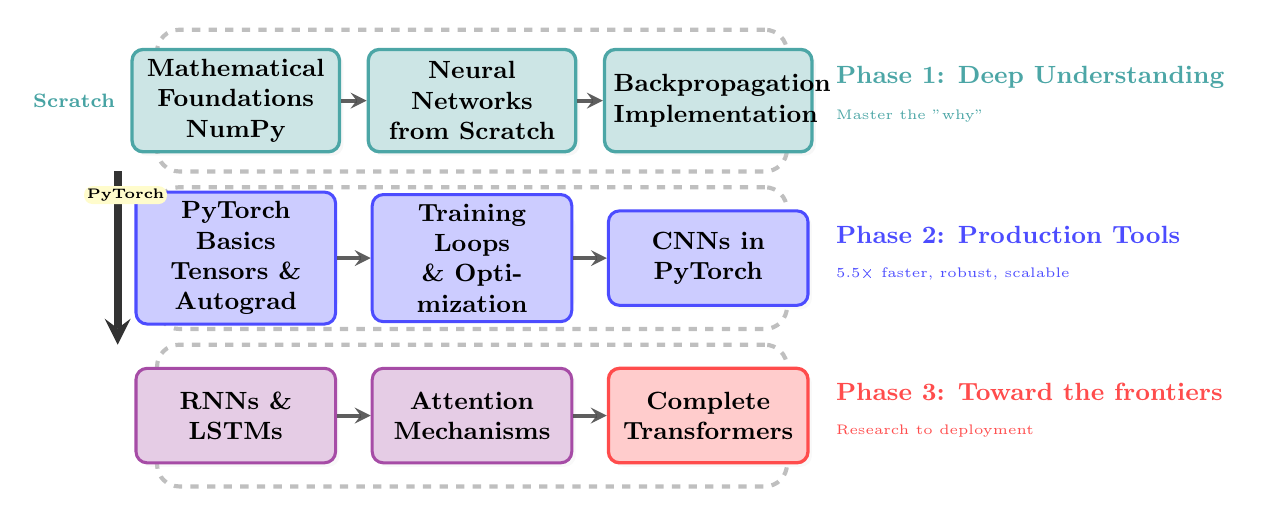
\begin{tikzpicture}[
  % Color-blind friendly node styles using Tol's palette
  foundational/.style={rectangle, draw=teal!70, fill=teal!20, text width=2.4cm, text centered, minimum height=1.3cm, rounded corners=4pt, font=\small\bfseries, line width=1.2pt},
  intermediate/.style={rectangle, draw=blue!70, fill=blue!20, text width=2.3cm, text centered, minimum height=1.2cm, rounded corners=4pt, font=\small\bfseries, line width=1.1pt},
  advanced/.style={rectangle, draw=violet!70, fill=violet!20, text width=2.3cm, text centered, minimum height=1.2cm, rounded corners=4pt, font=\small\bfseries, line width=1.1pt},
  expert/.style={rectangle, draw=red!70, fill=red!20, text width=2.3cm, text centered, minimum height=1.2cm, rounded corners=4pt, font=\small\bfseries, line width=1.2pt},
  % Arrow styles with better visibility
  primary/.style={thick, ->, >=stealth, black!70, opacity=0.9, line width=1.5pt},
  journey/.style={very thick, ->, >=stealth, black!80, line width=3pt},
  % Dashed rectangle style for each level
  levelbox/.style={rectangle, draw=gray!50, dashed, line width=1.5pt, rounded corners=8pt, minimum width=8cm, minimum height=1.8cm}
]

% Layer 1: Dashed rectangles for each level
\node[levelbox] at (0,4.2) {};
\node[levelbox] at (0,2.2) {};
\node[levelbox] at (0,0.2) {};

% Layer 2: Manual shadow rectangles (behind main boxes)
\node[rectangle, fill=black!15, fill opacity=0.2, text width=2.4cm, minimum height=1.3cm, rounded corners=4pt] at (-2.95,4.15) {};
\node[rectangle, fill=black!15, fill opacity=0.2, text width=2.4cm, minimum height=1.3cm, rounded corners=4pt] at (0.05,4.15) {};
\node[rectangle, fill=black!15, fill opacity=0.2, text width=2.4cm, minimum height=1.3cm, rounded corners=4pt] at (3.05,4.15) {};
\node[rectangle, fill=black!12, fill opacity=0.2, text width=2.3cm, minimum height=1.2cm, rounded corners=4pt] at (-2.95,2.15) {};
\node[rectangle, fill=black!12, fill opacity=0.2, text width=2.3cm, minimum height=1.2cm, rounded corners=4pt] at (0.05,2.15) {};
\node[rectangle, fill=black!12, fill opacity=0.2, text width=2.3cm, minimum height=1.2cm, rounded corners=4pt] at (3.05,2.15) {};
\node[rectangle, fill=black!12, fill opacity=0.2, text width=2.3cm, minimum height=1.2cm, rounded corners=4pt] at (-2.95,0.15) {};
\node[rectangle, fill=black!12, fill opacity=0.2, text width=2.3cm, minimum height=1.2cm, rounded corners=4pt] at (0.05,0.15) {};
\node[rectangle, fill=black!12, fill opacity=0.2, text width=2.3cm, minimum height=1.2cm, rounded corners=4pt] at (3.05,0.15) {};

% Layer 3: Main content boxes
\node[foundational] (math) at (-3,4.2) {Mathematical\\Foundations\\NumPy};
\node[foundational] (scratch) at (0,4.2) {Neural Networks\\from Scratch};
\node[foundational] (backprop) at (3,4.2) {Backpropagation\\Implementation};
\node[intermediate] (pytorch) at (-3,2.2) {PyTorch Basics\\Tensors \& Autograd};
\node[intermediate] (training) at (0,2.2) {Training Loops\\\& Optimization};
\node[intermediate] (cnns) at (3,2.2) {CNNs in\\PyTorch};
\node[advanced] (rnns) at (-3,0.2) {RNNs \&\\LSTMs};
\node[advanced] (attention) at (0,0.2) {Attention\\Mechanisms};
\node[expert] (transformers) at (3,0.2) {Complete\\Transformers};

% Layer 4: Horizontal progression arrows within each level
\draw[primary] (math) -- (scratch);
\draw[primary] (scratch) -- (backprop);
\draw[primary] (pytorch) -- (training);
\draw[primary] (training) -- (cnns);
\draw[primary] (rnns) -- (attention);
\draw[primary] (attention) -- (transformers);

% Layer 5: Single vertical progression arrow with transition highlight
\draw[journey] (-4.5,3.3) -- (-4.5,1.1);

% Add transition emphasis between Phase 1 and 2
\node[fill=yellow!20, rounded corners=3pt, font=\tiny\bfseries, inner sep=1pt] at (-4.4,3.0) {\shortstack{PyTorch}};

% Layer 6: Text labels (on top of everything)
% Skill level indicators with better positioning and background
\node[teal!80, font=\scriptsize\bfseries, anchor=west, fill=white, fill opacity=0.9, rounded corners=1pt, inner sep=2pt] at (-5.65,4.2) {Scratch};
\node[red!80, font=\scriptsize\bfseries, anchor=west, fill=white, fill opacity=0.9, rounded corners=1pt, inner sep=2pt] at (-5.65,0.2) {};

% Level labels on the right with benefits
\node[teal!70, font=\small\bfseries, anchor=west] at (4.5,4.5) {Phase 1: Deep Understanding};
\node[teal!70, font=\tiny, anchor=west] at (4.5,4.0) {Master the "why"};

\node[blue!70, font=\small\bfseries, anchor=west] at (4.5,2.5) {Phase 2: Production Tools};
\node[blue!70, font=\tiny, anchor=west] at (4.5,2.0) {5.5× faster, robust, scalable};

\node[red!70, font=\small\bfseries, anchor=west] at (4.5,0.5) {Phase 3: Toward the frontiers};
\node[red!70, font=\tiny, anchor=west] at (4.5,0.0) {Research to deployment};

\end{tikzpicture}